\chapter{Theoretische Problembetrachtung}
\label{chap:theorie}
\minitoc

%%%%%%%%%%%%%%%%%%%%%%%%%%%%%%%%%%%%%%%%%%%%%%%%%%%%%%%%%%%%%%%%%%%%%%%%%%%%%%%%
%%%%%%%%%%%%%%%%%%%%%%%%%%%%%%%%%%%%%%%%%%%%%%%%%%%%%%%%%%%%%%%%%%%%%%%%%%%%%%%%

\section{Erneuerbare Energien im Energieversorgungsnetz}

Die erneuerbaren Energien \"ubernehmen in Deutschland mit jedem Jahr einen
gr\"o\ss eren Anteil an der Elektrizit\"atsversorgung. Mehr als die H\"alfte
\todo{wo ist die Quelle?}der erneuerbaren Energie wird durch Wind und
Photovoltaik erzeugt. Diese Energiequellen sind jedoch in hohem Grad
witterungsabh\"angig und k\"onnen stark fluktuieren. Dadurch kann die Menge der
zur Verf\"ugung stehenden Energie von der Nachfrage zeitlich enorm abweichen.
Dies kann den  sicheren Betrieb des Stromnetzes bei einer konstanten Frequenz
von $50$ Hz gef\"arden. Zus\"atzliche Bereitstellung an Regelleistung wird
dadurch notwendig. Au\ss erdem erfolgt die Erstellung der Fahrpl\"ane f\"ur
den Einsatz der konventionellen Kraftwerke gezwungenerma\ss en auf den
fehlerbehafteten Vortagsprognosen \"uber die Menge an Leistung aus erneuerbaren
Energien. Die G\"ute der Prognose bestimmt dabei direkt den Regel- und den
Reservebedarf.

Eine exakte Prognose \"uber die Leistung aus Wind- und Photovoltaikanlagen kann
nur auf Grundlage exakter Wettervorhersagen erfolgen. In der Literatur wird eine
mittlere Genauigkeit f\"ur Day-Ahead Windleistungsprognosen von $7\,\%$
\cite{prognose_doctor} und f\"ur Leistungsprognose aus Photovoltaikanlagen im
Bereich von $3,5\,\%\,-\,4,4\,\%$ \cite{solarvorhersagung} angegeben.
Dar\"uberhinaus k\"onnen im Verlauf eines Tages zeitweise deutliche Abweichungen
von diesen Werten auftreten. Durch den gedrosselten Betrieb der Anlagen ist
eine M\"oglichkeit zur Kompensation der Prognosefehler gegeben. Der gedrosselte
Anteil kann dadurch jedoch nicht genutzt werden. Die Bereitstellung der
Regelleistung durch konventionelle oder andere Kraftwerke erscheint hier als
sinnvoll. Eine Alternative zu den obengenannten Methoden bieten Energiespeicher,
da sie bei \"Uberangebot Energie speichern k\"onnen und bei Unterversorgung
Energie in das Netz einspeisen k\"onnen.

Variable Gestalltung der Netzlast kann weiterhin zur Reduzierung der
obengenannten Problematik beitragen.

Dies bedeutet, dass beispielsweise Gro\ss verbraucher in Zeiten geringen
Energiebedarfs zeitweilig vom Netz genommen und die dadurch freiwerdenden
Kapazit\"aten anderwertig eingesetzt werden. Dies h\"atte zur Folge, dass sowohl
Regelungsverluste als auch der Regelungsaufwand verringert und somit Kosten
gespart werden k\"onnten. Es ist vorstellbar, dass Anlagen zur K\"alteerzeugung
aufgrund der thermischen Tr\"agheit zu g\"unstigen Zeiten die Temperatur
zus\"atzlich senken k\"onnen und zu ung\"unstigen Zeiten die K\"uhlt\"atigkeit
auf das Minimum herunterfahren. Hiermit ist also das Interesse begr\"undet, das
Lastverlagerungspotential in der K\"alteerzeugung zu untersuchen.

%%%%%%%%%%%%%%%%%%%%%%%%%%%%%%%%%%%%%%%%%%%%%%%%%%%%%%%%%%%%%%%%%%%%%%%%%%%%%%%%
%%%%%%%%%%%%%%%%%%%%%%%%%%%%%%%%%%%%%%%%%%%%%%%%%%%%%%%%%%%%%%%%%%%%%%%%%%%%%%%%

\section{K\"alteerzeugung im Supermarkt: Potentiale und Besonderheiten}

Im Mittel entfallen $60\,\%$\cite{leghart, EANRW} des Stromverbrauchs in einem
Supermarkt auf das Kühlen und Tiefkühlen von Produkten. Der durchschnittliche
Verbrauch in einem Supermarkt liegt zwischen 300 MWh und 500 MWh im
Jahr\cite{leghart}. In den kommenden Jahren sch\"atzt man das Wachstum des
gesamten K\"altebedarfs f\"ur Deutschland auf 100 \% \cite{probst}. Der Anteil
am Bedarf an elektrischer Energie vom Gesamtverbrauch eines Industrielandes für
Kälteerzeugung in den Supermärkten wird in der Literatur f\"ur  Australien mit
$1\, \%$ \cite{australia} und in Schweden mit $2\, \%$ \cite{doctor, EANRW}
angegeben. In Deutschland liegt der Verbrauch mit 6294 $GWh$ f\"ur das
Jahr 1999 bei rund $1,27\, \%$\cite{steilme}. Die Gr\"o\ss enordnung des
Verbrauchs f\"ur die Produktlagerung in Superm\"arkten und die M\"oglichkeit
diesen zeitlich zu verschieben, macht die Superm\"arkte f\"ur die Regelung
besonders interessant. Jedoch unterliegt der Einsatz bestimmten Beschr\"ankungen
und Randbedingungen.

Die Mindesthaltbarkeit f\"ur bestimmte Produkte kann nur durch Lagerung
dieser Produkte in f\"ur sie festgelegtem K\"uhltemperaturbereichen garantiert
werden. Dieser Temperaturbereich ist je nach Bedarf und Anwendung in
Normalk\"uhlung (NK\abvz{NK}{Normalk\"uhlung}) über 0$\grad$C und in
Tiefk\"uhlung (TK\abvz{TK}{Tiefk\"uhlung}) unter 0$\grad$C unterteilt. Auf der
nationalen und auch auf der internationalen Ebene existieren Auflagen, die die
maximale Temperaturen bei der Lagerung von Nahrungsmitteln vorschreiben. Die
fundamentale Verordnung ist die EG 853/2004. Aus der geht hervor, dass
normalgekühlte Produkte im Temperaturbereich von 0 bis $+8$$\grad$C je nach
Nahrungsmittel und tiefgekühlte Produkte mindestens bei $-18$$\grad$C gekühlt
werden müssen.

Die K\"alteerzeugung im Supermarkt kann r\"aumlich generell in zwei Bereiche
unterteilt werden, dem Verkaufsbereich und dem Warenlager. Au\ss erdem kommen
K\"uhleinheiten zum Einsatz, die einer Verbundk\"alteanlage angeh\"oren oder
steckerfertig zur Verf\"ugung stehen. Im Verkaufsbereich kommen \"uberwiegend
K\"uhltruhen im Tiefk\"uhlbereich und K\"uhltruhen und -regale im
Niederk\"uhlbereich zum Einsatz. Zur Ausstattung z\"ahlen Ger\"ate in offener
sowie durch T\"uren verschlie\ss barer Ausf\"uhrung. Gr\"o\ss tenteils werden
die offenen Modelle au\ss erhalb der \"Offnungszeiten durch Decken und Rollos
zwecks Energieeinsparung verschlossen.

%%%%%%%%%%%%%%%%%%%%%%%%%%%%%%%%%%%%%%%%%%%%%%%%%%%%%%%%%%%%%%%%%%%%%%%%%%%%%%%%
%%%%%%%%%%%%%%%%%%%%%%%%%%%%%%%%%%%%%%%%%%%%%%%%%%%%%%%%%%%%%%%%%%%%%%%%%%%%%%%%

\section{Objektorientierte Programmierung mit \matlab}
\label{sec:OOP}
Seit Ende des letzten Jahrhunderts herrscht in der Fachliteratur für Informatik
die Meinung, dass der Einsatz von objektorientierten Techniken Programme
hervorbringt, die im Vergleich \textit{einfacher erweiterbar, besser testbar}
und \textit{besser wartbar} sind. Dabei wird ein Verfahren angewendet, nachdem
große Systeme in kleinere Teile des Ganzen zerlegt werden. Programme lassen sich
dadurch im Allgemeinen mit weniger Aufwand und kleinerer
Fehlerwahrscheinlichkeit programmieren. Inspiriert durch die Vorgänge aus der
realen Welt, werden die Abläufe durch operierende Objekte dargestellt, die
Aufträge erledigen und vergeben können. Die wesentlichen Eigenschaften der
objektorientierten Programmierung, kurz OOP\abvz{OOP}{objektorientierte
Programmierung}, sind die Datenkapselung, die Polymorphie und die
Vererbung.\footnote{ Ausführliche Informationen dazu findet
man z.B. in \cite{OOP},\cite{pepperOOP},\cite{java} oder \cite{python}.}

%%%%%%%%%%%%%%%%%%%%%%%%%%%%%%%%%%%%%%%%%%%%%%%%%%%%%%%%%%%%%%%%%%%%%%%%%%%%%%%%
%%%%%%%%%%%%%%%%%%%%%%%%%%%%%%%%%%%%%%%%%%%%%%%%%%%%%%%%%%%%%%%%%%%%%%%%%%%%%%%%

\subsection*{Allgemeine Erl\"auterungen}
\begin{description}

	\item[Klasse] Eine Klasse ist ein Instrument der Programmierung zur
	Erfassung von charakteristischen Eigenschaften zusammenh\"angender
	Objekte. Die Definition der Strukturen der Objekte erfolgt durch
	Klassen.

	\item[Objekt] Ein Objekt ist ein konkretes Exemplar einer
	Klasse.

	\item[Eigenschaften] Eigenschaften sind Variablen, die f\"ur jedes
	Objekt existieren.

	\item[Methoden] Methoden sind objektlokale Funktionen.

	\item[Datenkapselung] Man spricht von Kapselung, wenn Objekte den
	Zugriff auf ihre Daten kontrollieren.

	\item[Polymorphie] K\"onnen unterschiedliche Objekte auf eine gleiche
	Nachricht unterschiedlich reagieren, spricht man von Polymorphie.

	\item[Vererbung] Die Vererbung erm\"oglicht durch Ver\"anderung der
	bestehenden Klassen neue Klassen zu erstellen. Die grundlegenden
	Programmteile der bestehenden Klasse werden zwangsl\"aufig
	\"ubernomen.

\end{description}

%%%%%%%%%%%%%%%%%%%%%%%%%%%%%%%%%%%%%%%%%%%%%%%%%%%%%%%%%%%%%%%%%%%%%%%%%%%%%%%%
%%%%%%%%%%%%%%%%%%%%%%%%%%%%%%%%%%%%%%%%%%%%%%%%%%%%%%%%%%%%%%%%%%%%%%%%%%%%%%%%

\subsection*{Erl\"auterungen zur OOP-Syntax\footnote{ Es werden nur
Schl\"usselw\"orter vorgestellt, die essentiell sind. Eine tiefgreifende
Darstellung w\"urde den Rahmen einer Studienarbeit bei Weitem \"ubersteigen.
Ausf\"uhrliche Informationen dazu findet man z.B. in \cite{matlab_kompakt} oder
\url{http://www.mathworks.com/help/}.}}

\begin{description}

	\item[classdef] Neue Klassen werden mit der Anweisung
	\lstinline$classdef$ eingeleitet. Der Name der Klasse wird unmittelbar
	nach der Anweisung eingetragen. Der Klassen-Block endet mit der
	Anweisung \lstinline$end$.
	\item[properties] Die Anweisung \lstinline$properties$ beginnt den
	Eigenschaften-Block. Abgeschlossen wird der Block mit \lstinline$end$.
	Innerhalb einer Klasse k\"onnen mehrere Bl\"ocke existieren. M\"ochte
	man das Verhalten eines Eigenschaften-Blocks zus\"atzlich ver\"andern,
	zum Beispiel neue Zugriffsarten oder Zugriffsrechte vergeben, ist der
	Einsatz von Attributen zweckm\"a\ss ig.
	\begin{lstlisting}[frame=none]
	properties (attribut1, attribut2, etc.)
	end
	\end{lstlisting}
	\item[methods] Die Anweisung \lstinline$methods$ beginnt den
	Methoden-Block und mit \lstinline$end$ wird er geschlossen. Analog zu
	dem Eigenschaften-Block k\"onnen in einer Klasse mehrere
	Methoden-Bl\"ocke existieren. M\"ochte man das Verhalten eines
	Methoden-Blocks zus\"atzlich ver\"andern, ist der Einsatz von Attributen
	zweckm\"a\ss ig.
	\begin{lstlisting}[frame=none]
	methods (attribut1, attribut2, etc.)
	end
	\end{lstlisting}


\end{description}

%%%%%%%%%%%%%%%%%%%%%%%%%%%%%%%%%%%%%%%%%%%%%%%%%%%%%%%%%%%%%%%%%%%%%%%%%%%%%%%%
%%%%%%%%%%%%%%%%%%%%%%%%%%%%%%%%%%%%%%%%%%%%%%%%%%%%%%%%%%%%%%%%%%%%%%%%%%%%%%%%

\subsection*{Klassen und Objekte mit \matlab}

Klassen werden in \matlab mit Hilfe einer Datei mit der Endung $.m$ definiert,
die den selben Namen wie die Klasse hat. Im Quelltextbeispiel
\matref{Klassendefinition} wird eine Beispielklasse \textbf{class\_name} mit
einem Eigenschaften-Block und einem Methoden-Block definiert. Die Datei muss
demnach \textbf{class\_name.m} hei\ss en. In die erste Zeile der Datei kommt die
Anweisung \lstinline$classdef$, die die Klasse einleitet. Werden der Klasse
zus\"atzliche Verhaltensmuster zugewiesen, folgt die Setzung der Attribute in
Klammern. Anschlie\ss end kommt der Name der Klasse. Wird die neue Klasse eine
durch Vererbung abgeleitete einer anderen Klasse, so folgt das Kleinerzeichen
und der Name der Superklasse. In den anschlie\ss enden Zeilen werden der
Eigenschaften-Block und der Methoden-Block definiert.

\begin{lstlisting}[float=h!,caption={Beispiel Klassendefinition},label={Klassendefinition}, frame=none]
	classdef (Attributes) class_name < super_class % class definition
		properties (Attributes) % first property block
			PropertyName = [];
		end % end of properties block
		% additionally here can be another properties block with 
		% specifying by another Attributes
		methods (Attributes) 
			function obj = class_name(obj,a) % consturctor
				obj.PropertyName = a;
			end
			function [X] = second_function(obj)
				X = obj.PropertyName + 1;
			end
		end
		% additionally here can be another methods block with 
		% specifying by another Attributes
	end % end of classdef block
\end{lstlisting}

Objekte einer Klasse werden durch eine Konstruktor-Methode erzeugt. Diese
Funktion wird im ersten Methoden-Block an erster Stelle definiert. Sie hat den
selben Namen wie die Klasse. \"Uber die Konstruktor-Funktion k\"onnen bereits
bei der Erzeugung der Objekte Werte an ausgew\"ahlte Attribute \"ubergeben
werden. Erfolgt der Aufruf einer Konstruktor-Funktion einer Klasse fehlerfrei,
so ist das Ergebnis des Aufrufes ein Objekt dieser Klasse. Der Aufruf eines
Konstruktors unterscheidet sich nicht von dem Aufruf gew\"ohnlicher
\matlab-Funktionen. Im folgenden Quelltextbeispiel wird im Command-Window durch
den Aufruf der Konstruktor-Funktion ein Objekt \textbf{object} der im
\matref{Klassendefinition} vorgestellten Klasse erzeugt.
\begin{lstlisting}[frame=none]
	>> object = class_name(input_data);
\end{lstlisting}

Methoden, die applikationsspezifische Operationen mit einem Datensatz
durchf\"uhren sollen, werden nach der Konstruktor-Funktion definiert.  Die
meisten dieser Funktionen nutzen das Objekt als Eingabeargument, zum Beispiel:
\lstinline{second_function(obj)}. Der Zugriff auf die Variablen der
Objekteigenschaften erfolgt durch Referenzierung auf das Objekt. Im
Quelltextbeispiel \matref{Klassendefinition} wird das wie folgt vorgestellt:
\lstinline{obj.PropertyName}. Wenn ein Zugriff auf Objektfunktionen erlaubt ist,
kann darauf wie folgt zugegriffen werden:

\begin{lstlisting}[frame=none]
	>> function_return = object.second_function;
\end{lstlisting}
\noindent Die Referenz auf den Namen des Objektes muss stets erfolgen.

%%%%%%%%%%%%%%%%%%%%%%%%%%%%%%%%%%%%%%%%%%%%%%%%%%%%%%%%%%%%%%%%%%%%%%%%%%%%%%%%
%%%%%%%%%%%%%%%%%%%%%%%%%%%%%%%%%%%%%%%%%%%%%%%%%%%%%%%%%%%%%%%%%%%%%%%%%%%%%%%%

\section{Einf\"uhrung in die K\"altetechnik}

An dieser Stelle wird ein knapper \"Uberblick über die mathematischen und
physikalischen Zusammenhänge gegeben, die bei der Entwicklung eines Modells
einer K\"alteanlage in einem Modellsupermarkt zwingend beachtet werden müssen.\\

In den Superm\"arkten werden K\"uhlger\"ate zur Lagerung der Ware bis zum
Verkauf an den Endkunden eingesetzt. Um die Haltbarkeit dieser Ware f\"ur den
Mindestzeitraum zu gew\"ahrleisten, wird sie bei niedrigen Temperaturen
gehalten. Körper mit unterschiedlicher Temperatur sind bestrebt, wenn sie
thermisch von einander nicht vollkommen isoliert sind, durch gegenseitige
Wechselwirkung ihre Temperaturen anzugleichen. Infolge dessen wird ein
Wärmegleichgewicht erreicht. Der nat\"urliche W\"armefluss findet
selbstst\"andig immer vom K\"orper mit der h\"oheren Temperatur in die Richtung des
K\"orpers mit der niedrigeren Temperatur statt. Um eine negative
Temperaturänderung herzustellen und diese auch zu halten, muss die eindringende
Wärmeenergie ständig in derselben Höhe abgeführt werden, damit die Temperatur
konstant bleibt. Diese Energiemenge pro Zeiteinheit wird als Kälteleistung
bezeichnet. Eine Abweichung von dieser Menge führt zum Steigen der Temperatur,
wenn weniger und zum Sinken der Temperatur wenn mehr abgeführt wird. Um diesen
Kühlkreislauf aufrecht zu erhalten, muss Leistung aufgewendet werden\footnote{
	Eine detailierte Beschreibung dieser Prozesse in einer
	Kompressionskälteanlage und Spezifikation ist nicht Gegenstand dieser
	Arbeit.  Ausführliche Informationen dazu findet man z.B.  in \cite{caro,
	doctor, TAB_A1}.}.

\begin{figure}[h]
\begin{center}
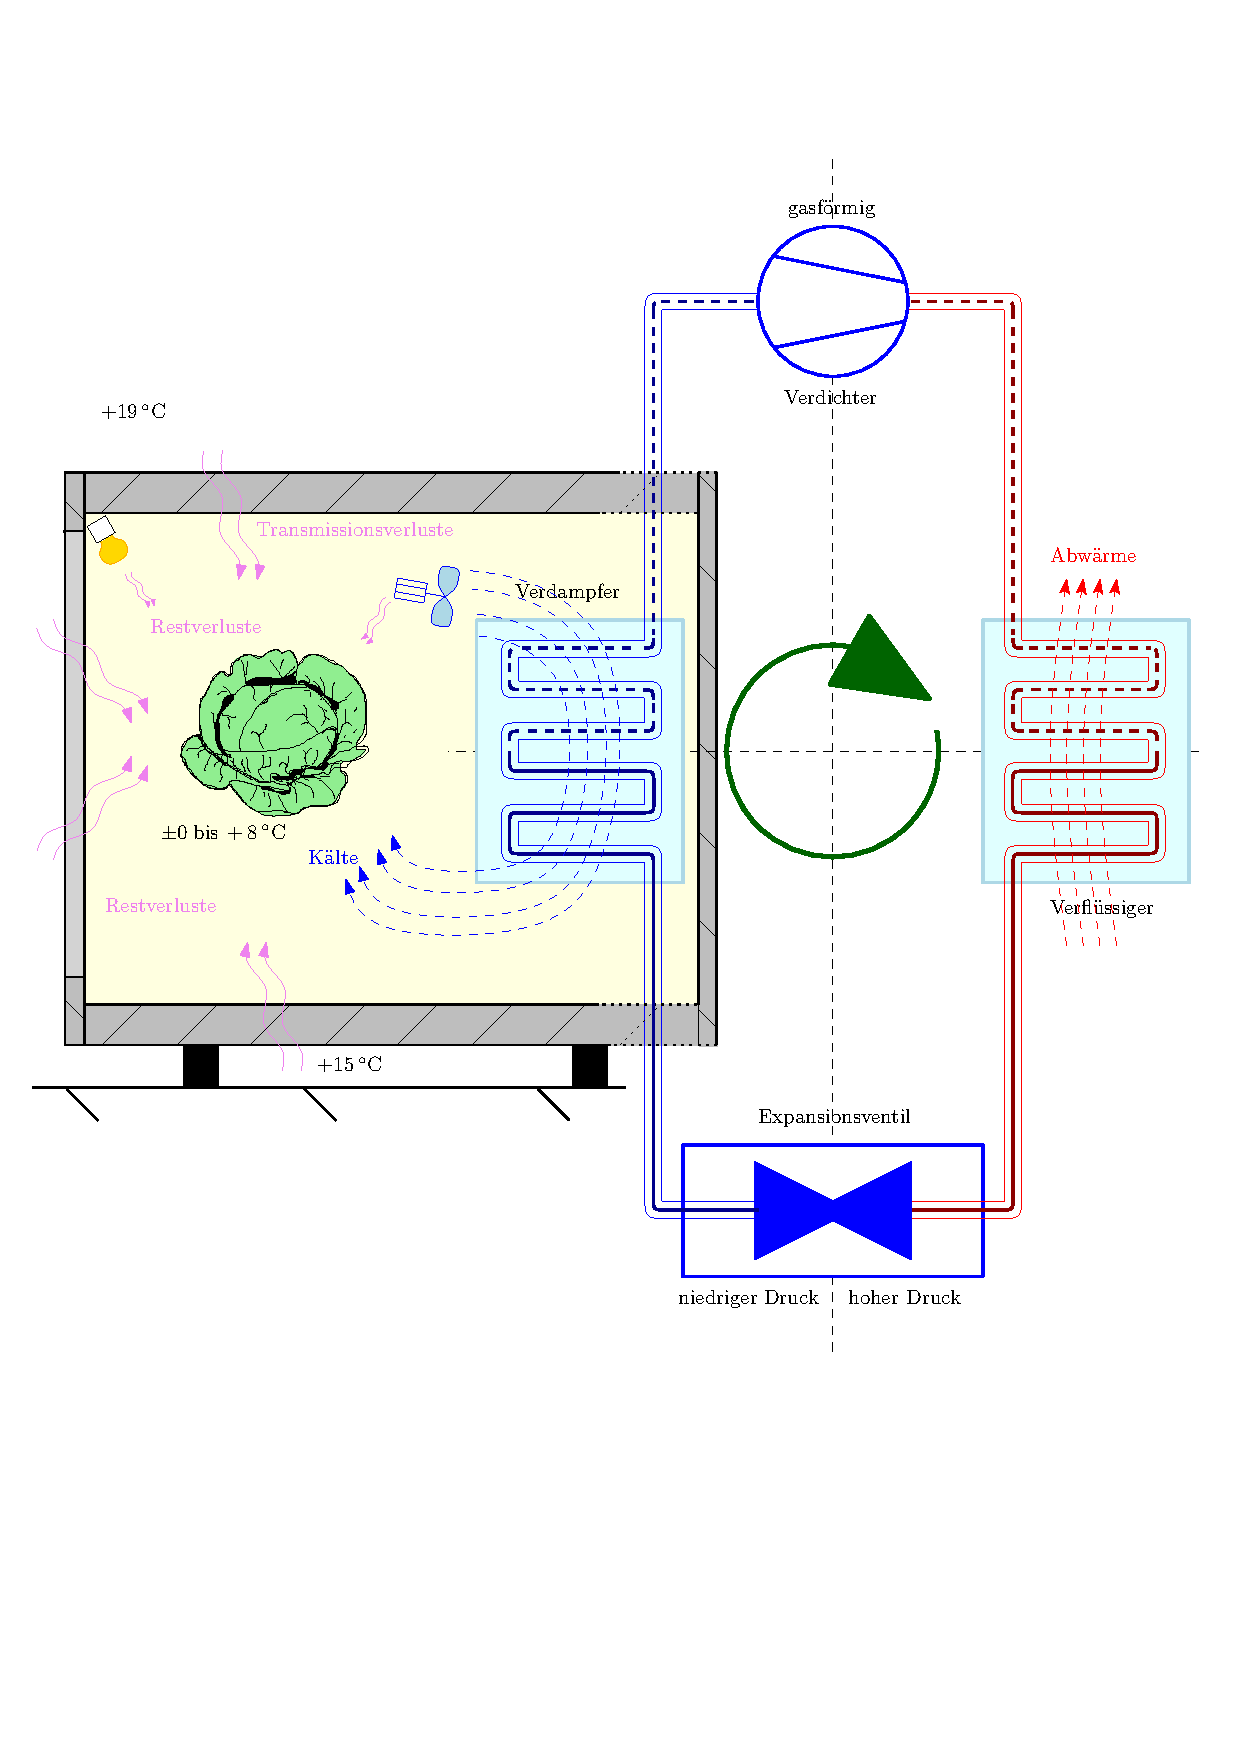
\includegraphics[scale=0.6]{/images/Theorie_Super/fridge}
\end{center}
\caption{Prinzipdarstellung Kompressionsk\"alteanlage}
\label{fig:prinz}
\end{figure}

In der \cref{fig:prinz} auf der Seite \pageref{fig:prinz} ist die
Prinzipdarstellung der weitverbreiteten Kompressionsk\"altemaschine zu sehen.
Die Ware, die symbolisch durch einen Kohlkopf dargestellt ist, wird mit einer
Temperatur zwischen $\pm 0$ und $+8\grad$C gelagert. Der Temperaturunterschied
zwischen dem Innen- und Au\ss enbereich ist ma\ss gebend f\"ur den Verlust an
K\"alte (W\"armeausgleich).  Der Ausgleich f\"uhrt dazu, dass K\"altenergie
f\"ur den Lagerungs- und K\"uhlungsprozess verloren geht.

Die Aufnahme der Wärmeenergie und der spezifischen Wärmekapazität dieser
Substanzmasse ergibt die Temperaturdifferenz $\Delta\:t$.

\begin{equation}
	\Delta\:t = \frac{Q}{m\cdot c}
\label{tdif}
\end{equation}

\begin{description}[\dth]

	\item[$\Delta\:t$] Temperaturdifferenz in Kelvin K
	\item[$Q$] Verlust an K\"alte in in kJ
	\item[$m$] Substanzmasse zur Aufnahme der K\"alteenergie in kg
	\item[$c$] Spezifische K\"altekapazit\"at (W\"armekapazit\"at) der
	Substanzmasse in $\mathrm{\frac{kJ}{kg \cdot K}}$

\end{description}
\vspace{0.5cm}

Die installierte Kälteleistung multipliziert mit der täglichen Betriebszeit muss
gleich dem stündlichen K\"altebedarf multipliziert mit der Tagesstundenzahl
sein.

\begin{equation}
	\pinstall = \frac{24}{ \tau_{B} }  \cdot \pkalt \label{pinstall}
\end{equation}

\begin{description}[\dth]

	\item[$\pinstall$] Installierte Kälteleistung in kW
	\item[$\tau_{B}$] Tägliche Betriebszeit in h
	\item[$\pkalt$] st\"undlicher Kälteleistungsbedarf in
	kW\todo{st\"undlicher!!! \"uberall}

\end{description}
\vspace{0.5cm}

Die Transmissionswärmeleistung wird aus der Multiplikation der Fläche
der wärmeübertragenden Wände mit ihrem spezifischen Wärmedurchgangskoeffizient
und der Temperaturdifferenz zwischen der Kühlraumtemperatur und der
Umgebungstemperatur berechnet.

\begin{equation}
	\ptrans = A \cdot k \cdot \Delta t
	\label{ptrans}
\end{equation}

\begin{description}[\dth]

	\item[$\ptrans$] Transmissionswärmeleistung in kW
	\item[$A$] Fläche in $\mathrm{m^2}$
	\item[$k$] Wärmedurchgangskoeffizient\todo{e zuviel} in $\mathrm{\frac{W}{m^2 \cdot
	K}}$
	\item[$\Delta\: t$] Temperaturdifferenz in K

\end{description}
\vspace{0.5cm}

Der Zusammenhang zwischen der aufgewendeten elektrischen Antriebsleistung $P$
eines Verdichters in einer Kompressionskälteanlage und der genutzten
st\"undlichen Kälteleistung ${\dot{Q}}_0$ wird durch die Kältezahl $\epsilon$
wiedergegeben.

\begin{equation}
	\epsilon = \frac{\pkalt}{P}
\label{epsilon}
\end{equation}

\begin{description}[\dth]

	\item[$\epsilon$] Leistungszahl (einheitenlos)
	\item[$\pkalt$] st\"undliche Kälteleistungsbedarf in kW
	\item[$P$] elektrische Verdichterantriebsleistung in einer
		Kompressionskälteanlage in kW

\end{description}
\vspace{0.5cm}

Die Öffnungszeit des Supermarkts hat einen spürbaren Einfluss auf die Größe der
K\"alteverluste. In der Literatur wird der Nachtverbrauch mit $10\,\%$ bis $20\,\%$
des Tagesverbrauchs angegeben\cite{kauffeld}.  In der Nacht fallen keine
zusätzlichen Verluste an, zum Beispiel durch Licht, Körperwärme oder
Türöffnungszeiten, sodass nur Transmissionsverluste bei der Berechnung beachtet
werden. Leistungsbedarf definiert die Menge an Leistung, der ben\"otigt wird, um
den Verlust an K\"alte zu ersetzen. Die Abweichung zwischen Tagesbedarf und
Nachtbedarf an Leistung wird im weiteren Verlauf Tagesmehrbedarf genannt.

\begin{equation}
	\dot{Q}_{Nacht}=\ptrans
\label{pnacht}
\end{equation}

\begin{description}[\dth]

	\item[$\pnacht$] Leistungsbedarf in der Nacht in kW
	\item[$\ptrans$] Transmissionswärmeleistung in kW

\end{description}
\vspace{0.5cm}


Der K\"alteleistungsbedarf am Tag ergibt sich aus der Summe des Tagesmehrbedarfs
und der Transmissionswärmeleistung. Aus Gründen der Vereinfachung wird der
Tagesmehrbedarf als weitgehend konstant angenommen.

\begin{equation}
	\ptag = \pmehr + \ptrans
\label{ptag}
\end{equation}

\begin{description}[\dth]

	\item[$\ptag$] Leistungsbedarf am Tag in kW
	\item[$\pmehr$] Tagesmehrbedarf am Tag in kW
	\item[$\ptrans$] Transmissionswärmeleistung in kW

\end{description}
\vspace{0.5cm}

Die Verlustk\"altememenge im K\"uhlbereich ist aufgrund der obengenannten
Gr\"unde je nach Tageszeit unterschiedlich.

\begin{equation}
	Q_v = \begin{cases}
	1h \cdot \pnacht, & \text{au\ss erhalb der \"Offnungszeiten}\\
	1h \cdot \ptag, & \text{innerhalb der \"Offnungszeiten}
	\end{cases}
\label{qv}
\end{equation}

\begin{description}[\dth]

	\item[$Q_v$] Verlustk\"altemenge in kJ
	\item[$\ptag$] Leistungsbedarf am Tag in kW
	\item[$\pnacht$] Leistungsbedarf in der Nacht in kW
	\item[$h$] Zeiteinheit f\"ur Stunden

\end{description}
\vspace{0.5cm}


Ist f\"ur eine K\"alteanlage der st\"undliche K\"alteleistungsbedarf bekannt, so
wird der Tagesmehrbedarf an K\"alteleistung ermittelt, indem vom Produkt des
K\"alteleistungsbedarfes mit dem Faktor f\"ur K\"altebedarfsabsenkung die
mittlere Transmissionswärmeleistung abgezogen wird.

\begin{equation}
	\pmehr = \pkalt \cdot K - \aptrans
\label{pmehr}
\end{equation}

\begin{description}[\dth]

	\item[$\pmehr$] Tagesmehrbedarf in kW
	\item[$\pkalt$] st\"undliche Kälteleistungsbedarf in kW
	\item[$K$] Faktor für Kältebedarfsabsenkung (einheitenlos)
	\item[$\aptrans$] mittlere Transmissionswärmeleistung in kW

\end{description}
\vspace{0.5cm}

Die Berechnung der mittleren Transmissionswärmeleistung erfolgt durch die
Multiplikation der Differenz zwischen der Umgebungstemperatur und der mittleren
Kühlraumtemperatur mit dem Wärmedurchgangskoeffizienten und der Fläche der
wärmeübertragenden Wände.

\begin{equation}
	\aptrans = A \cdot k \cdot \left( t_{amb} -
	\overline{t}_{KR} \right)
	\label{aptrans}
\end{equation}

\begin{description}[\dth]

	\item[$\aptrans$] mittlere Transmissionswärmeleistung in kW
	\item[$A$] Fläche in $\mathrm{m^2}$
	\item[$k$] Wärmedurchgangskoeffiziente in $\mathrm{\frac{W}{m^2 \cdot K}}$
	\item[$t_{amb}$] Umgebungstemperatur in $^{\circ}$ C
	\item[$\overline{t}_{KR}$] mittlere Kühlraumtemperatur in
		$^{\circ}$ C
\end{description}
\vspace{0.5cm}

Ist der Kälteleistungsbedarf nicht bekannt, wie zum Beispiel bei steckerfertigen
Geräten, kann der Mehrbedarf am Tag \"uber den Wert Verdichterarbeit pro 24
Stunden $\lverd$ für den gesamten Kälteverbraucher ermittelt werden.

Das Produkt aus dem spezifischen Energieverbrauch mit dem Faktor für
Kältebedarfsabsenkung, dem Verdichteranteil ergibt die Verdichterarbeit.
\begin{equation}
	v_{mod} = K \cdot v
\label{vmod}
\end{equation}
\begin{equation}
	\lverd = \lspez \cdot v_{mod}
\label{lverd}
\end{equation}

\begin{description}[\dth]

	\item[$\lverd$] Verdichterarbeit pro 24 Stunden in
	$\mathrm{\frac{kWh}{24h}}$
	\item[$\lspez$] spezifischer Energieverbrauch pro 24 Stunden in
		$\mathrm{\frac{kWh}{24h}}$
	\item[$K$] Faktor für Kältebedarfsabsenkung (einheitenlos)
	\item[$v$] Verdichteranteil (einheitenlos)
	\item[$v_{mod}$] modifizierter Verdichteranteil (einheitenlos)

\end{description}
\vspace{0.5cm}

Im Folgenden muss die Verdichterarbeit zum Ersetzen der zus\"atzlichen
K\"alteenergieverlustmenge in der \"Offnungszeit berechnet werden, die in einem
weiteren Schritt in Tagesmehrbedarf $\pmehr$ umgewandelt wird.

\begin{equation}
	\lmehr = \lverd - \frac{\aptrans}{\epsilon} \cdot 24
\label{lmehr}
\end{equation}

\begin{description}[\dth]

	\item[$\lmehr$] Verdichterarbeit zum Ersetzen der zus\"atzlichen
	K\"alteenergieverluste $\emehr$ in der \"Offnungszeit in kWh
	\item[$\lverd$] Verdichterarbeit pro 24 Stunden in
	$\mathrm{\frac{kWh}{24h}}$
	\item[$\aptrans$] mittlere Transmissionswärmeleistung in kW
	\item[$\epsilon$] Leistungszahl (einheitenlos)

\end{description}
\vspace{0.5cm}

Die Umrechnung von $\lmehr$ in $\pmehr$ erfolgt mit Hilfe der Leistungszahl
$\epsilon$. Die Verdichterarbeit $\lmehr$ wird mit $\epsilon$ multipliziert.
Es wird angenommen, dass der Mehrbedarf in den rund zw\"olf Stunden der
\"Offnungszeit entsteht.

\begin{equation}
	\pmehr = \frac{\lmehr}{12} \cdot \epsilon
\label{spmehr}
\end{equation}

\begin{description}[\dth]

	\item[$\pmehr$] Tagesmehrbedarf in kW
	\item[$\lmehr$] Verdichterarbeit zum Ersetzen der zus\"atzlichen
	K\"alteenergieverluste $\emehr$ in der \"Offnungszeit in kWh
	\item[$\epsilon$] Leistungszahl (einheitenlos)

\end{description}
\vspace{0.5cm}


